\subsection{Lambda system}
A traditional $\Lambda$-system is a quantum mechanical system with two decoupled 'ground states' and one 'excited state' coupled to both ground states. Such a state with two ground state could realize a qubit by letting the ground state act as $\ket{0}$ and $\ket{1}$.

\begin{figure}[H]
    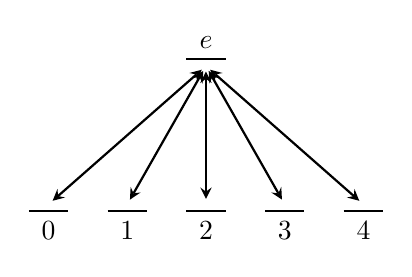
\begin{tikzpicture}[
      scale=0.5,
      level/.style={thick},
      virtual/.style={thick,densely dashed},
      trans/.style={thick,<->,shorten >=2pt,shorten <=2pt,>=stealth},
      classical/.style={thin,double,<->,shorten >=4pt,shorten <=4pt,>=stealth}]
      
    % Draw the energy levels.
    \draw[level] (6cm,0em) -- (7cm,0em) node[midway,above] {$\ket{e}$};
    \draw[level] (2cm,-11em) -- (3cm,-11em) node[midway,below] {$\ket{0}$};
    \draw[level] (4cm,-11em) -- (5cm,-11em) node[midway,below] {$\ket{1}$};
    \draw[level] (6cm,-11em) -- (7cm,-11em) node[midway,below] {$\ket{2}$};
    \draw[level] (8cm,-11em) -- (9cm,-11em) node[midway,below] {$\ket{3}$};
    \draw[level] (10cm,-11em) -- (11cm,-11em) node[midway,below] {$\ket{4}$};
    % Draw the transitions.
    
    \draw[trans] (6.5cm,-0.5em) -- (2.5cm,-10.5em) node[midway,left] {};
    \draw[trans] (6.5cm,-0.5em) -- (4.5cm,-10.5em) node[midway,left] {};
    \draw[trans] (6.5cm,-0.5em) -- (6.5cm,-10.5em) node[midway,left] {};
    \draw[trans] (6.5cm,-0.5em) -- (8.5cm,-10.5em) node[midway,left] {};
    \draw[trans] (6.5cm,-0.5em) -- (10.5cm,-10.5em) node[midway,left] {};
    %\draw[trans] (1cm,-2em) -- (2.5cm,8em) node[midway,left] {\ome{1}};
    %\draw[trans] (3.5cm,8em) -- (5cm,-8em) node[midway,right] {\Om{2}};
    %\draw[classical] (4.5cm,-8em) -- (1.5cm,-5em) node[midway,below] {\Ga{}};
    \end{tikzpicture}
    
    \caption{test figure}
\end{figure}

alfa $=$ $\frac{\pi}{2}\sin^{2}(\frac{\pi t}{T})$

beta $=$ $\eta(1 - \cos( \frac{\pi}{2}\sin^{2}(\frac{\pi t}{T}) ))$

alfa' $=$ $\frac{\pi^2}{2T}\sin(\frac{2\pi t}{T})$

beta' $=$ $\frac{\eta\pi^2}{2T}\sin(\frac{2\pi t}{T})\sin(\frac{\pi}{2}\sin^{2}(\frac{\pi t}{T}))$

\begin{equation*}
\Omega(t) = 2( (\frac{\eta\pi^2}{2T}\sin(\frac{2\pi t}{T})\sin(\frac{\pi}{2}\sin^{2}(\frac{\pi t}{T})))\cot(\frac{\pi}{2}\sin^{2}(\frac{\pi t}{T}))\sin(\eta(1 - \cos( \frac{\pi}{2}\sin^{2}(\frac{\pi t}{T}) )))
\end{equation*}
\begin{equation*}
+ \eta(1 - \cos( \frac{\pi}{2}\sin^{2}(\frac{\pi t}{T}) ))\cos(\eta(1 - \cos( \frac{\pi}{2}\sin^{2}(\frac{\pi t}{T}) ))) )
\end{equation*}



\subsection{Coupled excited states}
Hamiltonian of a ''double'' tripod
\begin{equation}
H(t) = \sum^2_{i = 1} \sum^3_{j = 1} \omega_{ij} \ket{j}\bra{e_i} + \text{h.c}
\end{equation}

Find dark states $H(t)\ket{d} = 0\ket{d} $ on form $\ket{d} = \sum_{k = 1}^3 d_k \ket{k}$
Result

\begin{equation}
\begin{aligned} &
d_1 = \frac{1}{\omega^{*}_{11}} \left(\omega^{*}_{12}\omega^{*}_{23}  - \omega^{*}_{13}\omega^{*}_{22} \right)
\\ &
d_2 = \frac{\omega^{*}_{13}\omega^{*}_{21}}{\omega^{*}_{11}} - \omega^{*}_{23}
\\ &
d_3 = \omega^{*}_{22} - \frac{\omega^{*}_{12}\omega^{*}_{21}}{\omega^{*}_{11}}
\end{aligned}
\end{equation}

Bright state $\bra{b}\ket{d} = 0$ 

\begin{equation}
\begin{aligned} &
\ket{b_1} = \omega_{11}\ket{1} + \omega_{12}\ket{2} + \omega_{13}\ket{3}
\\ &
\ket{b_2} = \omega_{21}\ket{1} + \omega_{22}\ket{2} + \omega_{23}\ket{3}
\end{aligned}
\end{equation}
Check if $\bra{b_1}\ket{b_2} = 0$? Holds if $\omega_{11} = -\frac{1}{\omega^{*}_{21}}\left(\omega^{*}_{12}\omega_{22} + \omega_{13}\omega^{*}_{23} \right)$


Change basis, 
\begin{equation}
T = \begin{pmatrix}
1 & 0 & 0 & 0 & 0 \\
0 & 1 & 0 & 0 & 0  \\
0 & 0 & \omega_{11} & \omega_{21} & d_1  \\
0 & 0 & \omega_{12} & \omega_{22} & d_2  \\
0 & 0 & \omega_{13} & \omega_{23} & d_3  \\
\end{pmatrix}
\end{equation}

New hamiltonian in $\{\ket{e_1}, \ket{e_2}, \ket{b_1}, \ket{b_2}, \ket{d} \}$ is 
\begin{equation}
H_d(t) = T^\dagger H(t) T = \left(\sum_{j = 1}^2 \sum_{k = 1}^3 \left( \omega_{jk} \right)^2 \ket{b_j}\bra{e_j}\right) + \left[\omega_{11}\omega_{12} + \omega_{12}\omega_{22} + \omega_{13}\omega_{23} \right]\left(\ket{b_2}\bra{e_1} + \ket{b_1}\bra{e_2}\right)\; + \;\text{h.c} 
\end{equation} 
\note{Double check this calculation.}


Subspace is  $\{\ket{e_1}, \ket{e_2}, \ket{b_1}, \ket{b_2} \}$ since $\ket{d}$ is decoupled.\\
Simplify notation, $\Omega_j = \sum_{k = 1}^3 \omega_{jk}^2$ and $\Gamma = \omega_{11}\omega_{12} + \omega_{12}\omega_{22} + \omega_{13}\omega_{23}$ now Hamiltonian looks like 
\begin{equation}
H_d = \sum_{j = 1}^2 \Omega_j \ket{b_j}\bra{e_j} + \Gamma\left(\ket{b_2}\bra{e_1} + \ket{b_1}\bra{e_2} \right) + \; \text{h.c}
\end{equation}
\\
Now find a ''dark path'' $\ket{D_i(t)}$ such that $\bra{D_i(t)}H_d(t)\ket{D_i(t)} = 0$, for $i = 1,2$
\\ Set
\begin{equation}
\begin{aligned} &
 \ket{D_1} = a_1\ket{b_1} + a_2\ket{3} + a_3\ket{e_1}
 \\ &
 \ket{D_2} = c_1\ket{b_2} + c_2\ket{3} + c_3\ket{e_2}
 \end{aligned}
\end{equation}

and


\vspace{3cm}
NEW TRY

\begin{equation}
H(t) = \sum^2_{i = 1} \sum^3_{j = 1} \omega_{ij} \ket{j}\bra{e_i} + \text{h.c}
\end{equation}

New dark state 
\begin{equation}
\ket{d} = d_1\ket{1} + d_2\ket{2}
\end{equation}
with $d_1 = -(\omega_{12}^{*} + \omega_{22}^{*})$, $d_2 = (\omega_{11}^{*} + \omega_{21}^{*})$
\note{There exists no dark state on this form ($d_1 = d_2 = 0$)}

bight state 
\begin{equation}
\ket{b} = -d_2^{*}\ket{1} + d_1^{*}\ket{2}
\end{equation}

\textbf{CRITERA?} $\omega_{11}\omega_{22} = \omega_{12}\omega_{21} \implies \frac{\omega_{11}}{\omega_{12}} = \frac{\omega_{21}}{\omega_{22}}$

change basis to $\{e_1, e_2, 3, b, d\}$
\begin{equation}
T = \begin{pmatrix}
1 & 0 & 0 & 0 & 0 \\
0 & 1 & 0 & 0 & 0  \\
0 & 0 & 0 & -d_2^{*} & d_1  \\
0 & 0 & 0 & d_1^{*} & d_2  \\
0 & 0 & 1 & 0 & 0  \\
\end{pmatrix}
\end{equation}


New hamiltonian 
\begin{equation}
H_d = \left(\sum_{j = 1}^{2} \omega_{j3}\ket{3}\bra{e_j} + \sigma_j\ket{b}\bra{e_j} \right) + \text{h.c}
\end{equation}
with 
$$
\sigma_1 = \omega_{12}d_1^{*} - \omega_{11}d_2^{*} = -\omega_{12}(\omega_{12} + \omega_{22}) - \omega_{11}(\omega_{11} + \omega_{21})
$$
$$
\sigma_2 = \omega_{21}d_1^{*}-\omega_{12}d_2^{*} = -\omega_{23}(\omega_{12} + \omega_{22}) - \omega_{12}(\omega_{11} + \omega_{21})
$$
\\
Now find a ''dark path'' $\ket{D_i(t)}$ such that $\bra{D_i(t)}H_d(t)\ket{D_i(t)} = 0$, for $i = 1,2$
\\ Set
\begin{equation}
\begin{aligned} &
 \ket{D_1} = a_1\ket{b} + a_2\ket{3} + a_3\ket{e_1}
 \\ &
 \ket{D_2} = c_1\ket{b} + c_2\ket{3} + c_3\ket{e_2}
 \end{aligned}
\end{equation}
Assume that $\ket{b_2} = \Delta\ket{b_1}$

\begin{equation}
\begin{aligned} &
 \ket{D_1} = \cos\alpha\cos\beta (((e^{-i\varphi})))\ket{b_1} - \cos\alpha\sin\beta\ket{3} - i\sin\alpha\ket{e_1}
 \\ &
 \ket{D_2} = \cos\alpha\cos\beta (((e^{-i\varphi})))\ket{b_2} - \cos\alpha\sin\beta\ket{3} - i\sin\alpha\ket{e_2}
 \end{aligned}
\end{equation}

then $\bra{D_1}\ket{D_2} = 0 \implies \bra{b_1}\ket{b_2} = - \tan^2\beta \implies \Delta = -i\tan\beta$ 
\begin{equation}
\begin{aligned}&
\bra{D_i}H_d\ket{D_i} = \left[\sigma_1^{*} + \sigma_2^{*} - \sigma_i\right]\Delta_i\cos\beta + \omega_{i3}\sin\beta = 0
\\ &
\implies \omega_{i3} = \Delta_i(\sigma_i - \sigma_1^{*} - \sigma_2^{*})\cot\beta
\end{aligned}
\end{equation}



\vspace{3cm}

NEW NEW TRY!\\

\begin{equation}
H(t) = \sum^2_{i = 1} \sum^3_{j = 1} \omega_{ij} \ket{j}\bra{e_i} + \text{h.c}
\end{equation}

Dark state

\begin{equation}
\begin{aligned} &
d_1 = -\left(\omega^{*}_{22} + \frac{\omega^{*}_{12}\omega^{*}_{23}}{\omega^{*}_{13}} \right)
\\ &
d_2 = \left(\omega^{*}_{21} + \frac{\omega^{*}_{11}\omega^{*}_{23}}{\omega^{*}_{13}}\right)
\\ &
d_3 = \frac{1}{\omega^{*}_{13}}\left( \omega^{*}_{21}\omega^{*}_{12} - \omega^{*}_{11}\omega^{*}_{22}\right)
\end{aligned}
\end{equation}
bright state 
\begin{equation}
\ket{b} = -d_2^{*}\ket{1} + d_1^{*}\ket{2}
\end{equation}


\begin{equation}
H_d = \left(\sum_{j\ = 1}^{2} \omega_{j3}\ket{3}\bra{e_j} + \sigma_j\ket{b}\bra{e_j} \right) + \text{h.c}
\end{equation}

$$
\sigma_1 = -\frac{\omega_{23}}{\omega_{13}}\left(\omega_{12}^2 + \omega_{11}^2 \right) - \omega_{11}\omega_{21} - \omega_{12}\omega_{22}
$$
$$
\sigma_2 = -\frac{\omega_{23}}{\omega_{13}}\left(\omega_{12}\omega_{22} + \omega_{11}\omega_{21}\right) - \left(\omega_{12}^2 + \omega_{22}^2\right)
$$
Then computations follow as before with new coeffcients.
\newpage

\begin{equation}
H = \sum_{j = 1}^{2}\alpha_j \ket{\alpha_j}\bra{e_j} + \sum_{i = 1}^{2} \omega_{ji} \ket{i}\bra{e_j} + \;\text{h.c}
\end{equation}
in new basis
\begin{equation}
H_d = \sum_{j = 1}^2 -\alpha_j^2 - \sum_{i = 1}^{2}\omega_{ji}^{2}\ket{b_j}\bra{e_j} -(\omega_{11}\omega_{21} + \omega_{12}\omega_{22})(\ket{b_2}\bra{e_1} + \ket{b_1}\bra{e_2}) + \; \text{h.c}
\end{equation}
simplify 
\begin{equation}
H_d = \sum_{j = 1}^2 \sigma_j\ket{b_j}\bra{e_j} + \Gamma (\ket{b_2}\bra{e_1} + \ket{b_1}\bra{e_2}) + \; \text{h.c}
\end{equation}

\begin{equation}
\begin{aligned} &
 \ket{D_1} = \cos\alpha\cos\beta e^{-i\varphi_1}\ket{b_1} - \cos\alpha\sin\beta\ket{\alpha_1} - i\sin\alpha\ket{e_1}
 \\ &
 \ket{D_2} = \cos\alpha\cos\beta e^{-i\varphi_2}\ket{b_2} - \cos\alpha\sin\beta\ket{\alpha_2} - i\sin\alpha\ket{e_2}
 \end{aligned}
\end{equation}

\begin{equation}
\bra{D_1}\ket{D_2} = \cos^2\alpha \cos^2\beta e^{+i(\varphi_2 - \varphi_1)}\bra{b_1}\ket{b_2} == 0 \textbf{?}
\end{equation}
holds if
\begin{equation}
\bra{b_1}\ket{b_2} = \omega_{11}^{*}\omega_{21}^{} + \omega_{12}^{*}\omega_{22}^{} = 0
\end{equation}

\newpage

NEW, hopefully last, try

The system \begin{figure}[H]
    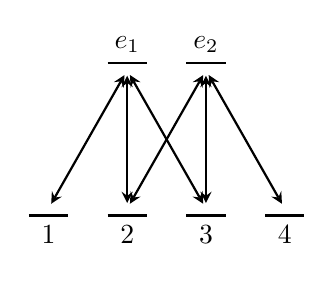
\begin{tikzpicture}[
      scale=0.5,
      level/.style={thick},
      virtual/.style={thick,densely dashed},
      trans/.style={thick,<->,shorten >=2pt,shorten <=2pt,>=stealth},
      classical/.style={thin,double,<->,shorten >=4pt,shorten <=4pt,>=stealth}]
      
    % Draw the energy levels.
    \draw[level] (6cm,0em) -- (7cm,0em) node[midway,above] {$\ket{e_1}$};    

    \draw[level] (4cm,-11em) -- (5cm,-11em) node[midway,below] {$\ket{1}$};
    \draw[level] (6cm,-11em) -- (7cm,-11em) node[midway,below] {$\ket{2}$};
    \draw[level] (8cm,-11em) -- (9cm,-11em) node[midway,below] {$\ket{3}$};
    \draw[level] (10cm,-11em) -- (11cm,-11em) node[midway,below] {$\ket{4}$};
    % Draw the transitions.
    
   
    \draw[trans] (6.5cm,-0.5em) -- (4.5cm,-10.5em) node[midway,left] {};
    \draw[trans] (6.5cm,-0.5em) -- (6.5cm,-10.5em) node[midway,left] {};
    \draw[trans] (6.5cm,-0.5em) -- (8.5cm,-10.5em) node[midway,left] {};

    
       
   
    \draw[trans] (8.5cm,-0.5em) -- (6.5cm,-10.5em) node[midway,left] {};
    \draw[trans] (8.5cm,-0.5em) -- (8.5cm,-10.5em) node[midway,left] {};
    \draw[trans] (8.5cm,-0.5em) -- (10.5cm,-10.5em) node[midway,left] {};


    \draw[level] (8cm,0em) -- (9cm,0em) node[midway,above] {$\ket{e_2}$};
    \end{tikzpicture}
    
    \caption{test figure}
\end{figure}

has a dark state $\ket{d}$ on the form 
\begin{equation}
\ket{d} = c_1\ket{1} + c_2\ket{2} + c_3\ket{3},\;\; |c_1|^2 + |c_2|^2 + |c_3|^2 = 1
\end{equation}

There exists two orthogonal bright states on the form 

\begin{equation}
\begin{aligned} &
\ket{b_1} = N_1 \left(x\ket{1} + c_2\ket{2} + c_3\ket{3} \right)
\\ &
\ket{b_2} = N_2 \left(-c_3^{*}\ket{2} + c_2^{*}\ket{3} \right)
\end{aligned}
\end{equation}

One can see that
$\bra{b_1}\ket{b_2} = \bra{d}\ket{b_1} 0$, find $x$ such that $\bra{d}\ket{b_1} = 0$.

After finding $x$ and normalizing the result is 
\begin{equation}
\begin{aligned}&
\ket{d} = c_1\ket{1} + c_2\ket{2} + c_3\ket{3}
\\ &
\ket{b_1} = \frac{|c_1|}{\sqrt{1-|c_1|^2}} \left(\left(c_1 - \frac{1}{c_1^{*}}\right)\ket{1} + c_2\ket{2} + c_3\ket{3} \right)
\\ &
\ket{b_2} =  \frac{1}{\sqrt{1-|c_1|^2}} \left(-c_3^{*}\ket{2} + c_2^{*}\ket{3} \right)
\end{aligned}
\end{equation}

The hamiltonian in the space spanned by $\{e_1, e_2, b_1, b_2, 4, d\}$ is given by 
\begin{equation}
H_d = \frac{\Omega_1(t)}{2}e^{-i\phi_1} \ket{b_1}\bra{e_1} + \frac{\Omega_2(t)}{2}e^{-i\phi_2} \ket{b_2}\bra{e_2} + \frac{\Omega_3(t)}{2}\ket{4}\bra{e_2} + \; \text{h.c}
\end{equation}

Two dark paths $\ket{D_i}$ exists such that  $\bra{D_i}H_d\ket{D_i} = 0, \; i=1,2$, on the form

\begin{equation}
\begin{aligned}&
\ket{D_1} = \alpha_1\ket{b_1} + \beta_1\ket{e_1}
\\&
\ket{D_2} = \alpha_2\ket{b_2} + \beta_2\ket{e_2} + \gamma\ket{4}
\end{aligned}
\end{equation}
A choice would be, given two functions, $u(0) = u(T) = v(0) = v(T) = 0$,
\begin{equation}
\begin{aligned}&
\alpha_1 = \cos u(t)
\\&
\beta_1 = e^{i(\phi_1 + \frac{\pi}{2})}\sin u(t)
\\&
\alpha_2 = \cos u \cos v e^{-i\phi_2}
\\&
\beta_2 = -i\sin u
\\&
\gamma = -\cos u\sin v
\end{aligned}
\end{equation}

the coeffcients of the dark state could be parametrized by 4 angles, $\chi, \xi, \theta, \varphi$ 

\begin{equation}
\begin{aligned}&
c_1 = e^{i\chi}\sin \theta \cos \varphi, 
\\&
c_2 = e^{i\xi} \sin \theta \sin \varphi,
\\&
c_3 = \cos \theta.
\end{aligned}
\end{equation}

Now to find the parameters $\Omega_1(t), \Omega_2(t), \Omega_3(t)$, this can be done by reverse engineering by solving the schrödinger equation for $\ket{D_1}, \ket{D_2}$, 

\begin{equation}
\begin{aligned}&
i\pdv{}{t}\ket{D_1(t)} = H_d\ket{D_1(t)}
\\&
i\pdv{}{t}\ket{D_2(t)} = H_d\ket{D_2(t)}
\end{aligned}
\end{equation}
a calculation yields
\begin{equation}
\begin{aligned}&
\Omega_1(t) = -2\dot{u}
\\ &
\Omega_2(t) = 2\left(\dot{v}\cot u\sin v + \dot{u}\cos v \right)
\\ &
\Omega_3(t) = 2\left(\dot{v}\cot u\sin v - \dot{u}\sin v \right)
\end{aligned}
\end{equation}

Split time evol. into two parts.
The relevant part of the time evolution operator is
\begin{equation}
\begin{aligned}&
U_1 = \ket{d}\bra{d} -i\ket{e_1}\bra{b_1} -i\ket{e_2}\bra{b_2},\; \phi_1 = \phi_2 = 0
\\&
U_2 = \ket{d}\bra{d} +ie^{i\gamma_1}\ket{b_1}\bra{e_1} +ie^{i\gamma_2}\ket{b_2}\bra{e_2},\; \phi_1 = -\gamma_1,\; \phi_2 = -\gamma_2
\end{aligned}
\end{equation}

The complete operator is then given by 
\begin{equation}
U = U_2U_1 = \ket{d}\bra{d} + e^{i\gamma_1}\ket{b_1}\bra{b_1} + e^{i\gamma_2}\ket{b_2}\bra{b_2}
\end{equation}
Then $U$ is unitary in the computational subspace $\{d,b_1,b_2\}$, since $UU^{\dagger} = U^{\dagger}U = \mathbbm{1}$ 


One can set $u(t) = \frac{\pi}{2}\sin^2\frac{\pi t}{T}$ and $v(t) = \eta\left[1 - \cos u(t)\right]$

Now $U$ can be determined by the 6(?) real parameters $\chi, \xi, \theta, \varphi, \gamma_1, \gamma_2$ as $U(\chi, \xi, \theta, \varphi, \gamma_1, \gamma_2)$ 





